\documentclass[11pt]{article}

\usepackage[utf8]{inputenc}
\usepackage{geometry} 
\usepackage{amsmath,amsthm,amssymb,graphicx,mathtools,tikz,hyperref,multicol,cancel,enumitem,booktabs,float,pgfplots,multirow,mathrsfs,textcomp,gensymb,soul,changepage,threeparttable}
\usepackage[italian]{babel}
\usepackage{hyphenat}
\hyphenation{mate-mati-ca recu-perare}
\usetikzlibrary{positioning}
\pgfplotsset{compat=1.14}

\newcommand{\n}{\mathbb{N}}
\newcommand{\z}{\mathbb{Z}}
\newcommand{\q}{\mathbb{Q}}
\newcommand{\cx}{\mathbb{C}}
\newcommand{\real}{\mathbb{R}}
\newcommand{\field}{\mathbb{F}}
\newcommand{\ita}[1]{\textit{#1}}
\newcommand{\com}[2]{#1\backslash#2}
\newcommand{\oneton}{\{1,2,3,...,n\}}
\newcommand{\idea}[1]{\begin{gather*}#1\end{gather*}}
\newcommand{\ef}{\ita{f} }
\newcommand{\eff}{\ita{f}}
\newcommand{\proofs}[1]{\begin{proof}#1\end{proof}}
\newcommand{\inv}[1]{#1^{-1}}
\newcommand{\setb}[1]{\{#1\}}
\newcommand{\en}{\ita{n }}
\newcommand{\vbrack}[1]{\langle #1\rangle}
\newcommand{\qRa}{\quad \Rightarrow \quad}
\newcommand{\smaca}[1]{\textbf{\textsc{#1}}}

\newenvironment{theorem}[2][Teorema]{\begin{trivlist}
		\item[\hskip \labelsep {\bfseries #1}\hskip \labelsep {\bfseries #2.}]}{\end{trivlist}}
\newenvironment{lemma}[2][Lemma]{\begin{trivlist}
		\item[\hskip \labelsep {\bfseries #1}\hskip \labelsep {\bfseries #2.}]}{\end{trivlist}}
\newenvironment{exercise}[2][Esercizio]{\begin{trivlist}
		\item[\hskip \labelsep {\bfseries #1}\hskip \labelsep {\bfseries #2.}]}{\end{trivlist}}
\newenvironment{proposition}[2][Proposizione]{\begin{trivlist}
		\item[\hskip \labelsep {\bfseries #1}\hskip \labelsep {\bfseries #2.}]}{\end{trivlist}}
\newenvironment{corollary}[2][Corollario]{\begin{trivlist}
		\item[\hskip \labelsep {\bfseries #1}\hskip \labelsep {\bfseries #2.}]}{\end{trivlist}}

\hypersetup {
	colorlinks,
	linkcolor=black
}

\graphicspath{{img/}}

\geometry{
	top=2cm,
	bottom=2cm,
	left=1.5cm,
	right=1.5cm
}

\begin{document}
	\setlength{\parindent}{0pt}
	\title{\vspace{-4em}{\large Algoritmi e Protocolli per la Sicurezza} \\
		Project Work}
	\author{Gerardo Selce - IEE22700089 \\
			Andrea Savastano - IEE22700086}
	\date{10/05/2026}
	\maketitle
	
	\vspace{-2em}\par\noindent\rule{\textwidth}{0.4pt}
	\begin{center}
		{\Large\sc Sistema per le votazioni}
	\end{center}
	\par\noindent\rule{\textwidth}{0.4pt}
	
	
	
	\tableofcontents
	\newpage
	
	
	\section{Introduzione}
	Questo elaborato definisce la progettazione e la descrizione di un protocollo di sicurezza per la realizzazione di un referendum binario digitale. Il protocollo da realizzare sarà utilizzato nell'ambito di votazioni universitarie, di conseguenza non dovrà essere eseguito in contesti particolarmente critici come delle votazioni nazionali. Quindi, alcune vulnerabilità o limitazioni non ammissibili in contesti particolarmente complessi saranno considerate accettabili nel contesto universitario scelto. \\ \\
L'elaborato è suddiviso in quattro sezioni. Il \textbf{Work Package 1} descrive in generale il modello del sistema, definendo gli attori coinvolti, i possibili avversari e le proprietà che si vogliono rispettare. Il \textbf{Work Package 2} mostra il protocollo progettato partendo dal modello definito al Work Package 1. Nel \textbf{Work Package 3} si analizza la sicurezza del protocollo proposto e infine il \textbf{Work Package 4} spiega i dettagli implementativi del protocollo progettato.
	
	\section{Work Package 1}
	\subsection{Attori del sistema}
Gli attori onesti inclusi nel sistema utilizzano il protocollo sicuro per completare il processo di votazione, e sono quattro.
\paragraph{User (U):} L'utente è l'entità del sistema che rappresenta l'elettore legittimato a votare. Quindi il suo obiettivo è quello di contattare il Server per inviare il proprio voto, ossia la sua preferenza sul referendum binario, scegliendo tra \textit{"SI"} e \textit{"NO"}.\\
L'utente vuole essere certo che il suo voto sia anonimo, in modo tale che nessun malintenzionato possa compromettere la comunicazione per scoprire la sua preferenza, e si aspetta che il voto resti segreto anche successivamente.\\
Inoltre l'entità in esame confida che il suo voto raggiunga la destinazione e che gli arrivi una conferma dell'avvenuta registrazione del suo voto e che sia integro all'interno del Server. In caso contrario desidera sapere che non è stato registrato a causa di qualsiasi errore del sistema, in modo tale che possa riprovare in seguito.\\
L'utente si aspetta che nessun malintenzionato utilizzi la sua identità per votare al suo posto, altrimenti l'utente perde la possibilità di votare e si compromette il sistema.\\
Quindi tale elettore legittimato deve avere una prova della propria identità, in modo tale da poter dimostrare al Server di essere un utente legittimo.

\paragraph{Server (S):} L'entità Server è incaricata di contare i voti degli utenti per determinare il risultato finale, senza riconoscere la vera identità del votante. L'entità in esame è quindi incaricata di mantenere anonimi i voti, in modo tale che nessun malintenzionato possa scoprire le preferenze degli utenti.\\
Il Server vuole essere certo che i voti che riceve siano autentici, ossia che provengano da utenti legittimi, e che non siano stati alterati durante la trasmissione.\\
L'entità in esame è incaricata di mantenere anonimi i voti, in modo tale che nessun malintenzionato possa scoprire le preferenze degli utenti.\\
L'attore è anche incaricato di registrare correttamente i voti e di garantire che non vengano registrati voti non validi.

\paragraph{Authenticator (A):} L'authenticator è l'entità che si interpone tra lo user che vuole votare e il Server che deve conservare le preferenze degli elettori. Il suo scopo è quello di controllare l'identità dell'entità che desidera votare, quindi controlla l'autenticità dell'utente in modo tale che possa essere considerato un elettore legittimato a partecipare al referendum.\\
Quindi è un vero e proprio proxy di sicurezza che rappresenta l'intermediario nella comunicazione tra lo user e il server per il processo di votazione.

\paragraph{CA :} 


\subsection{Threat model e Asset}


\subsection{Requisiti del sistema e priorità}
\begin{table}[H]
	\centering
	\small
	\renewcommand{\arraystretch}{1.4} % Aumenta l'altezza delle righe per leggibilità
	\begin{tabularx}{\textwidth}{l X c c c}
		\toprule
		\rowcolor{headergray}
		\textbf{Classe} & \textbf{Metodo (Tipo)} & \textbf{Complessità} & $\bm{WMC_{classe}}$ & $\bm{WMC_{classe}}$ \\ 
		\midrule
		
		\textbf{Library} & Library() \textit{\footnotesize (C)} & Low & 1 & 11\\
		& searchBooks(...) \textit{\footnotesize (I)} & Average & 9 \\
		& viewUsers() \textit{\footnotesize (S)} & Low & 1 \\
		\addlinespace[0.5em] \hline \addlinespace[0.5em]
		
		\textbf{Book} & Book(...) \textit{\footnotesize (C)} & Low & 1 & 1 \\
		\addlinespace[0.5em] \hline \addlinespace[0.5em]
		
		\textbf{Reservation} & Reservation(...) \textit{\footnotesize (C)} & Average & 4 & 4 \\
		\addlinespace[0.5em] \hline \addlinespace[0.5em]
		
		\textbf{User} & User(...) \textit{\footnotesize (C)} & Low & 1 & 57 \\
		& register(...) \textit{\footnotesize (M)} & High & 20 \\
		& login(...) \textit{\footnotesize (M)} & Average & 16 \\
		& logout(...) \textit{\footnotesize (M)} & High & 20 \\
		\addlinespace[0.5em] \hline \addlinespace[0.5em]
		
		\textbf{Staff} & Staff() \textit{\footnotesize (C)} & Low & 1 & 102 \\
		& addBook(...) \textit{\footnotesize (M)} & Average & 16 \\
		& updateBook(...) \textit{\footnotesize (M)} & High & 20 \\
		& removeBook(...) \textit{\footnotesize (M)} & Average & 16 \\
		& viewAllReservations() \textit{\footnotesize (S)} & Low & 1 \\
		& approveReservation(...) \textit{\footnotesize (M)} & Average & 16 \\
		& cancelReservation(...) \textit{\footnotesize (M)} & Average & 16 \\
		& sendReminder(...) \textit{\footnotesize (M)} & Average & 16 \\
		\addlinespace[0.5em] \hline \addlinespace[0.5em]
		
		\textbf{Reg. User} & RegisteredUser(...) \textit{\footnotesize (C)} & Low & 1 & 46 \\
		& reserveBook(...) \textit{\footnotesize (M)} & High & 20 \\
		& returnBook(...) \textit{\footnotesize (M)} & Average & 16 \\
		& viewReservedBooks() \textit{\footnotesize (I)} & Average & 9 \\
		\addlinespace[0.5em] \hline \addlinespace[0.5em]
		
		\textbf{Admin} & Administrator() \textit{\footnotesize (C)} & Low & 1 & 53 \\
		& manageUsers(...) \textit{\footnotesize (M)} & High & 20 \\
		& assignRole(...) \textit{\footnotesize (M)} & Average & 16 \\
		& deleteUser(...) \textit{\footnotesize (M)} & Average & 16 \\
		
		\bottomrule
	\end{tabularx}
	\caption{Analisi dettagliata WMC per classi e metodi (Legenda: C=Constructor, S=Selector, M=Modifier, I=Iterator).}
\end{table}

\subsection{Assunzioni del sistema}
	
	\section{Work Package 2}
	\subsection{Fase preliminare del sistema}

\begin{enumerate}
	\item \textbf{Certificazione della Certificate Authority}: poichè la certificate chain del nostro sistema è composta da una sola certificate authority, questa funge da root ed è in grado di autocertificarsi. Quindi, il primo passo è generare il certificato Cert(CA) della certificate authority e distribuirlo ai membri del sistema (server e authority).
	\item \textbf{Certificazione del Server}: 
		\begin{enumerate}
			\item Il server genera una coppia di chiavi (privata $sk_S$, pubblica $pk_S$).
			\item Il server chiede alla CA di certificare il messaggio (ID, $pk_S$), in cui l'ID è il nome DNS del server.
			\item La CA verifica che il server appartenga effettivamente all’infrastruttura autorizzata del sistema di voto universitario e che sia stato approvato dagli amministratori del sistema. 
			\item La CA genera una firma digitale del messaggio $\sigma = Sign_{sk_{CA}}(ID,\ pk_S)$.
			\item La CA unisce firma e dati, costruendo il certificato Cert(S) = ($\sigma$, ID, $pk_S$).
			\item La CA restituisce il certificato al server.
		\end{enumerate}
	\item \textbf{Certificazione dell'Authority}:
		\begin{enumerate}
			\item L'authority genera una coppia di chiavi (privata $sk_A$, pubblica $pk_A$).
			\item L'authority chiede alla CA di certificare il messaggio (ID, $pk_A$), in cui l'ID è il nome DNS dell'authority.
			\item La CA verifica che l'authority appartenga effettivamente all’infrastruttura autorizzata del sistema di voto universitario e che sia stata approvata dagli amministratori del sistema. 
			\item La CA genera una firma digitale del messaggio $\sigma = Sign_{sk_{CA}}(ID,\ pk_A)$.
			\item La CA unisce firma e dati, costruendo il certificato Cert(A) = ($\sigma$, ID, $pk_A$).
			\item La CA restituisce il certificato all'authority.
		\end{enumerate}
	\item \textbf{Scambio dei certificati}:
		\begin{itemize}
			\item Il server trasmette il suo certificato Cert(S) all'authority,
			\item L'authority trasmette il suo certificato al server.
		\end{itemize}	
	\item \textbf{Eventuale revoca dei certificati}:
		\begin{itemize}
			\item Se viene revocato il certificato del server, viene ripetuta la fase di certificazione del server e scambio dei certificati.
			\item Se viene revocato il certificato dell'authority, viene ripetuta la fase di certificazione dell'authority e scambio dei certificati.
		\end{itemize}
\end{enumerate}


\subsection{Fase certificato utente}
\begin{enumerate}
	\item L'utente genera una coppia di chiavi (privata $sk_U$, pubblica $pk_U$).
	\item L'utente chiede alla CA di certificare il messaggio (ID, $pk_U$), in cui l'ID è la matricola universitaria dell'utente. (qualcuno potrebbe fingersi qualcun altro).
	\item La CA verifica che la matricola ricevuta è valida.
	\item La CA genera una firma digitale del messaggio $\sigma = Sign_{sk_{CA}}(ID,\ pk_U)$.
	\item La CA unisce firma e dati, costruendo il certificato Cert(U) = ($\sigma$, ID, $pk_U$).
	\item La CA restituisce il certificato all'utente.
\end{enumerate}


\subsection{Fase handshake}


\subsection{Fase trasmissione voto}



	
	\section{Work Package 3}
	\subsection{Analisi delle proprietà di sicurezza}


\paragraph{Autenticità}:
Ogni Utente intenzionato a votare possiede un certificato digitale valido firmato dalla Certificate Authority. L'Authenticator verifica la validità del certificato e infine verifica la firma sul voto cifrato. Solo l'Utente in possesso della chiave privata $sk_U$ può produrre una firma valida, quindi un attaccante non può impersonare un elettore senza compromettere la sua chiave privata. \\
La proprietà è garantita solo se assumiamo che, in fase di richiesta certificato utente (2.2), tutti gli Utenti inseriscano nel campo Subject del certificato non firmato la propria matricola corretta. Se così non fosse, chiunque potrebbe fingersi qualcun'altro.

\paragraph{Unicità}:
La proprietà di unicità è garantita dall'Authenticator attraverso la struttura dati VoterMap, che mantiene traccia degli elettori che hanno già votato. In particolare, l'identificativo dell'elettore viene rappresentato mediante l'hash della sua chiave pubblica $H(pk_U)$. Quando un nuovo voto viene ricevuto, l'Authenticator verifica se tale identificativo è già presente nella mappa. In caso affermativo, la richiesta viene immediatamente rifiutata; in caso contrario il voto viene accettato e l'identificativo viene inserito nella struttura. Questo meccanismo impedisce a un utente legittimo di votare più volte utilizzando lo stesso certificato e la stessa coppia di chiavi. \\
La proprietà è garantita assumendo che l'Authenticator operi correttamente, che la VoterMap non venga alterata da soggetti esterni e che un elettore non possa ottenere più certificati validi associati alla stessa votazione.

\paragraph{Integrità}:
La proprietà di integrità è garantita mediante l'utilizzo delle firme digitali su tutti i messaggi critici del protocollo. In particolare, il voto trasmesso dall'Utente all'Authenticator è accompagnato da una firma digitale generata mediante la chiave privata dell'Utente. L'Authenticator verifica tale firma utilizzando la corrispondente chiave pubblica ottenuta dal certificato dell'Utente. Analogamente, il messaggio inoltrato dall'Authenticator al Server viene firmato dall'Authenticator e verificato dal Server. \\
La proprietà è garantita assumendo che le chiavi private degli attori onesti (Utente, Authenticator e Server) rimangano segrete. \\
L'integrità del contenuto del voto durante la trasmissione è garantita dal protocollo. Tuttavia, il protocollo assume che il Server, una volta decifrato il voto, si comporti in maniera semi-honest e non alteri volontariamente il risultato dello scrutinio. Pertanto l'integrità del risultato finale dipende parzialmente da tale assunzione di fiducia.


\paragraph{Segretezza}:
La proprietà di segretezza viene garantita mediante l'utilizzo della cifratura asimmetrica sul voto trasmesso dall'utente. Infatti l'Utente, oltre a trasmettere il voto cifrato con la sua chiave pubblica da salvare sull'Authenticator, trasmette il voto cifrato utilizzando la chiave pubblica del Server e quindi non decifrabile dall'Authenticator. L'Authenticator quindi sa che l'Utente ha votato ma non può ottenere l'informazione relativa al voto. D'altro canto, l'Authenticator inoltra il voto cifrato al Server il quale riceve esclusivamente il voto cifrato e le informazioni necessarie a verificarne la provenienza dall'Authenticator. Non riceve certificati dell'Utente, chiavi pubbliche dell'Utente o altri identificativi che consentano di risalire direttamente all'elettore che ha espresso il voto. \\
La proprietà è quindi garantita sotto l'assunzione che l'Authenticator e il Server si comportino come entità semi-honest e non colludano. Se dovessero colludere, l'Authenticator potrebbe inviare al Server anche l'identità dell'Utente votante oltre al suo voto. Questo permetterebbe al Server di associare l'identità dell'Utente al suo voto espresso.

\paragraph{Verificabilità Individuale}:
La proprietà di verificabilità individuale è garantita dalla struttura VoterMap mantenuta dall'Authenticator e dalla procedura di verifica del voto. Infatti, per ogni elettore che ha votato, l'Authenticator conserva una coppia costituita dall'identificativo dell'utente $H(pk_U)$ e dal voto cifrato con la chiave pubblica dell'utente $c = Enc_{pk_U}(v)$. Successivamente, l'Utente può autenticarsi presso l'Authenticator e richiedere il recupero del proprio voto cifrato. \\
Una volta ricevuto il voto cifrato associato al proprio identificativo, l'Utente può decifrarlo utilizzando la propria chiave privata $sk_U$ ed ottenere il voto in chiaro. Confrontando il voto ottenuto con quello che intendeva esprimere, l'Utente può verificare che il voto registrato dal sistema corrisponda effettivamente alla propria scelta elettorale. \\
La proprietà è garantita assumendo che l'Authenticator conservi correttamente la VoterMap e restituisca all'Utente il voto effettivamente associato al suo identificativo. Inoltre, si assume che il Server operi in modo semi-honest e non alteri i voti ricevuti dall'Authenticator prima dello scrutinio. In caso contrario, l'Utente potrebbe verificare correttamente il voto conservato dall'Authenticator ma non quello effettivamente conteggiato dal Server.

\paragraph{Verificabilità Universale}:
La proprietà di verificabilità universale non è completamente garantita dal protocollo proposto. Al termine dello scrutinio il Server pubblica il risultato finale della votazione e il numero totale di voti validi, firmando digitalmente tali informazioni. Chiunque può quindi verificare l'autenticità e l'integrità del risultato pubblicato mediante la verifica della firma digitale del Server. \\
Tuttavia, il protocollo non prevede la pubblicazione dei voti registrati né meccanismi crittografici che consentano a soggetti esterni di ricostruire autonomamente il conteggio effettuato dal Server. Di conseguenza, un osservatore esterno può verificare che il risultato pubblicato provenga effettivamente dal Server, ma non può verificare indipendentemente che ciascun voto sia stato conteggiato correttamente durante lo scrutinio. \\
La proprietà è quindi soddisfatta solo parzialmente e dipende dall'assunzione che il Server si comporti come un'entità semi-honest. Un Server malevolo potrebbe infatti alterare il conteggio finale dei voti senza che un osservatore esterno possa rilevare tale comportamento utilizzando esclusivamente le informazioni pubblicate dal protocollo.


\subsection{Analisi degli attacchi del Threat Model}


\paragraph{Identity Theft}:

\paragraph{Spoofing Authenticator}:

\paragraph{Spoofing Server}:

\paragraph{Man-in-the-Middle}:

\paragraph{Replay Attack}:

\paragraph{Eavesdropping}:

\paragraph{Traffic Analysis}:

\paragraph{Authenticator Curioso}:

\paragraph{Server Curioso}:


\subsection{Analisi delle assunzioni di fiducia}


	
	\section{Work Package 4}
	\subsection{Struttura ed Esecuzione del Progetto}
All'interno della cartella principale del progetto è presente la cartella \texttt{source}, che contiene il codice sorgente del progetto, organizzato in 4 cartelle principali: \texttt{actors}, \texttt{crypto}, \texttt{models} e \texttt{simulation}.

\begin{figure}[H]
	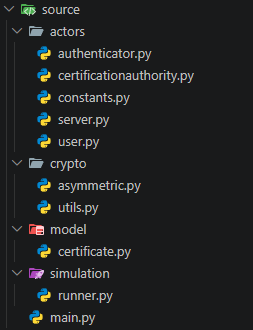
\includegraphics{./img/struttura_progetto.png}
	\centering
\end{figure}
In particolare:
\begin{itemize}
	\item \textbf{actors:} contiene le classi che rappresentano i vari attori del sistema (Utente, Authenticator, Server, CA).

	\item \textbf{crypto:} contiene le classi che implementano le primitive crittografiche utilizzate nel sistema (ad esempio, firme digitali, cifratura).

	\item \textbf{model:} contiene una classe wrapper per i certificati digitali, che semplifica la gestione dei certificati all'interno delle funzioni delle classi degli attori, nascondendo i dettagli di implementazione dei certificati digitali.\\
	In un'implementazione futura può essere ragionevole creare le classi wrapper per le strutture dati (come la VoterMap, il buffer dell'Authenticator e la lista dei nonce del server) e per i pacchetti scambiati tra gli attori, in modo da semplificare e rendere ancora più leggibile la comunicazione tra gli attori.

	\item \textbf{simulation:} contiene la funzione runner che simula l'intero processo di voto, dalla registrazione degli utenti alla pubblicazione dei risultati, per uno o più utenti, con la possibilità di visualizzare l'output dettagliato o sintetico del processo di voto. 
\end{itemize}

All'interno della cartella source del progetto è presente il file \texttt{main.py}, che permette di eseguire la simulazione. Quindi per avviare la simulazione dalla cartella principale del progetto, è possibile eseguire il comando:
\begin{lstlisting}
$ python ./source/main.py
\end{lstlisting}

\subsection{Simulazione e Output}
La simulazione crea un certo numero di utenti (specificato nel file \texttt{main.py}) e simula l'intero processo di voto per ciascun utente, dalla registrazione alla pubblicazione dei risultati. Solo per il primo utente viene mostrato l'output dettagliato del processo di voto, mentre per gli altri utenti viene mostrato solo l'output sintetico per non riempire il terminale.\\
Ciascuna fase definita dal protocollo viene mostrata in output con il dettaglio di tutte le operazioni eseguite da ciascun utente, evidenziando l'attore che sta eseguendo l'operazione col suo colore di riferimento ripreso dal diagramma di sequenza del protocollo.\\

Di seguito è riportato l'esempio di output dettagliato per la fase preliminare del sistema:
\begin{figure}[H]
	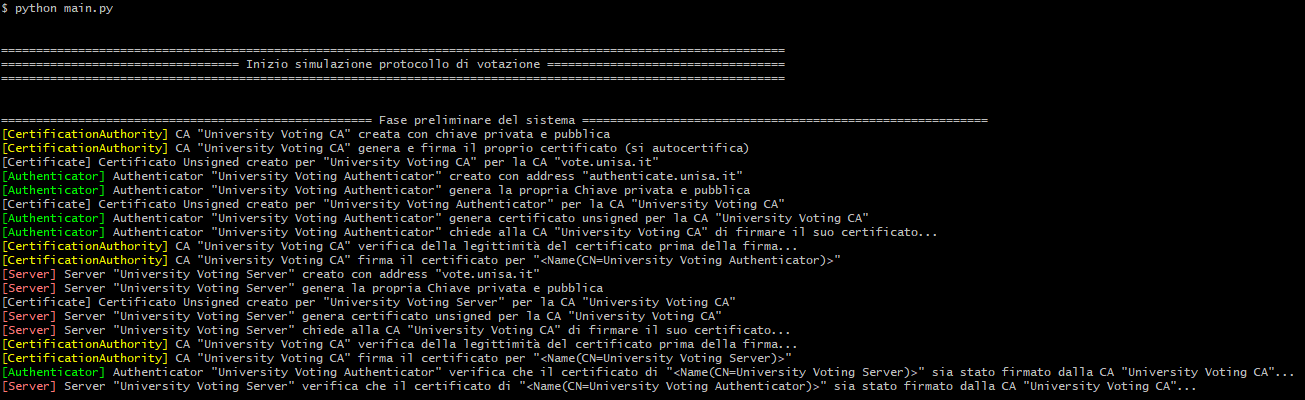
\includegraphics[width=1\textwidth]{./img/output_fase_preliminare.png}
	\centering
\end{figure}

Di seguito è riportato l'esempio di output della creazione di utenti:
\begin{figure}[H]
	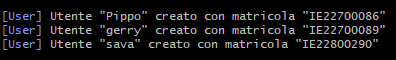
\includegraphics[width=.7\textwidth]{./img/output_user_creation.png}
	\centering
\end{figure}

Di seguito è riportato l'esempio di output dettagliato della simulazione per l'utente "Pippo" (il primo utente creato nella simulazione), differenziando le varie fasi del protocollo.\\
Fase certificato utente:
\begin{figure}[H]
	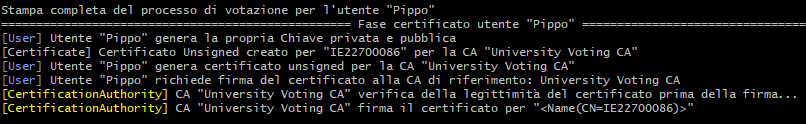
\includegraphics[width=1\textwidth]{./img/output_fase_certificato_utente.png}
	\centering
\end{figure}

Fase di handshake:
\begin{figure}[H]
	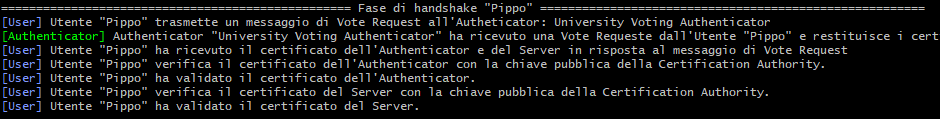
\includegraphics[width=1\textwidth]{./img/output_fase_handshake.png}
	\centering
\end{figure}

Fase trasmissione voto:
\begin{figure}[H]
	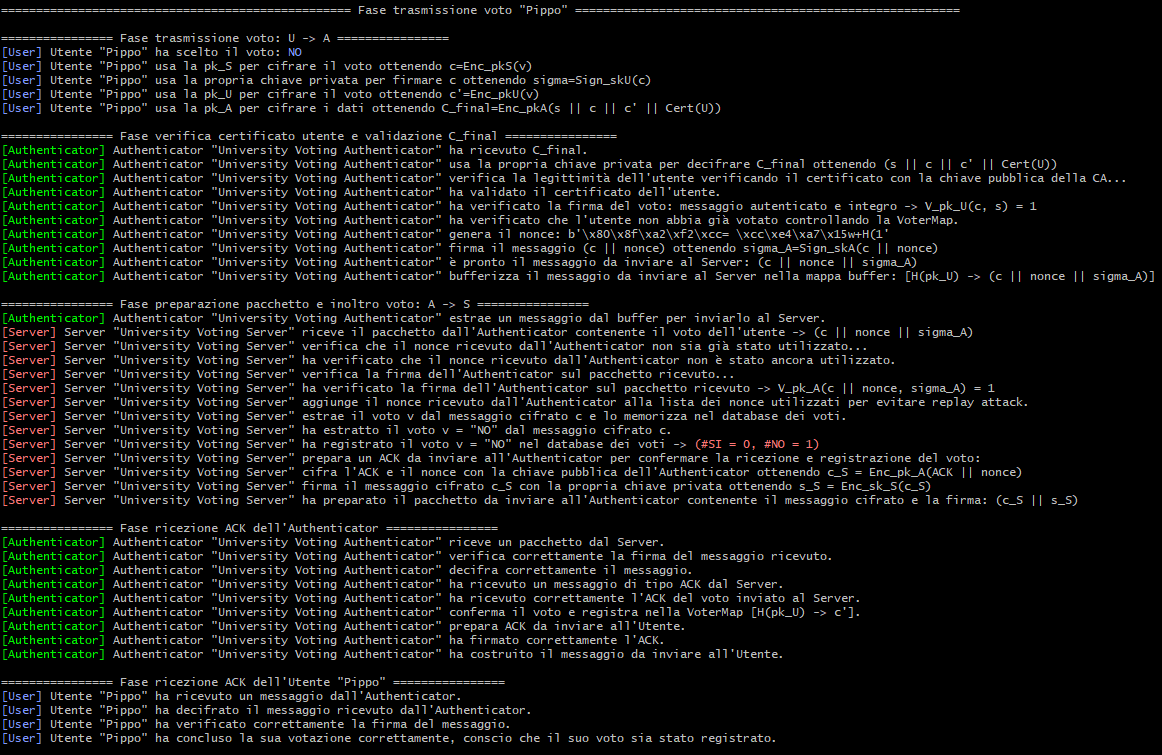
\includegraphics[width=1\textwidth]{./img/output_fase_trasmissione_voto.png}
	\centering
\end{figure}

Di seguito è riportato l'esempio di output della verifica individuale dei voti da parte dell'utente "Pippo":
\begin{figure}[H]
	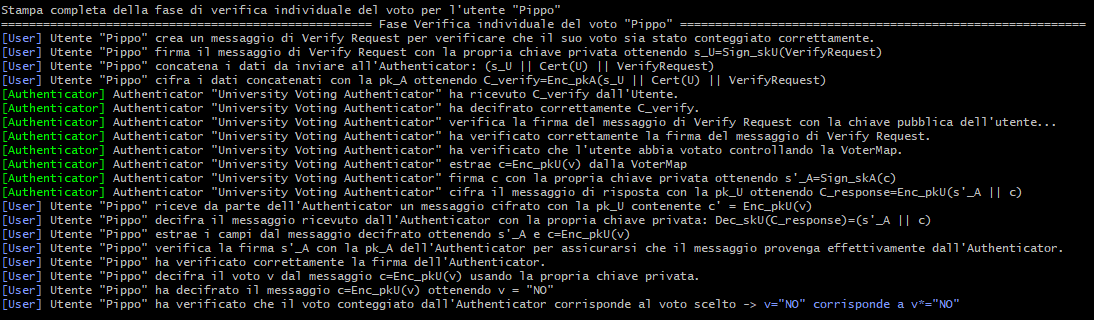
\includegraphics[width=1\textwidth]{./img/output_verifica_individuale.png}
	\centering
\end{figure}

Di seguito è riportato l'esempio di output della verifica universale dei voti da parte degli utenti:
\begin{figure}[H]
	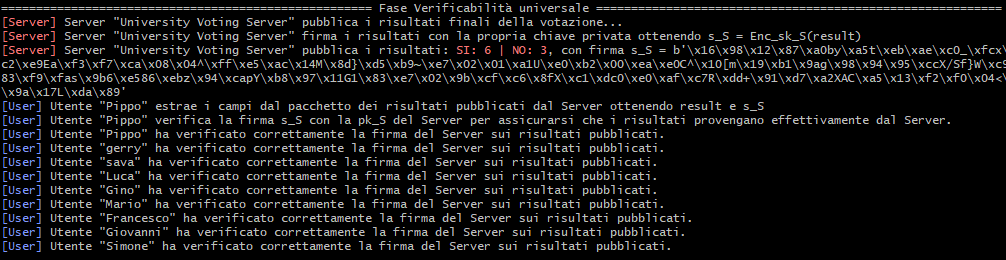
\includegraphics[width=1\textwidth]{./img/output_verifica_universale.png}
	\centering
\end{figure}

\subsection{Problema e miglioria futura}
Nella fase di trasmissione voto del protocollo stabilito, l'utente deve creare il cifrato $C_{final} = \text{Enc}_{pk_A}(\sigma \| c\| c'\| \text{Cert(U)})$ da inoltrare al server. Secondo il protocollo, il cifrato $C_{final}$ deve essere creato utilizzando l'algoritmo di cifratura asimmetrica RSA-OAEP, che prevede l'utilizzo di un padding randomico. Tuttavia si presenta l'impossibilità di cifrare interamente la concatenazione di $\sigma \| c\| c'\| \text{Cert(U)}$ con RSA-OAEP, in quanto la dimensione del messaggio da cifrare supera la dimensione massima consentita per la cifratura con RSA-OAEP (che dipende dalla dimensione della chiave pubblica utilizzata).\\
La scelta didattica per risolvere questo problema è stata quella di dividere il messaggio da cifrare in più parti, cifrando ciascuna parte separatamente con RSA-OAEP, ottenendo in questo modo un vettore di cifrati che rappresenta il cifrato finale $C_{final}$.\\
Ovviamente questa soluzione non è ottimale, in quanto se i singoli blocchi cifrati non sono crittograficamente legati tra loro, un attaccante sulla rete (attacco Man-in-the-Middle) potrebbe eliminare, duplicare o riordinare i blocchi cifrati alterando il messaggio finale senza invalidare le singole decifrature. Un altro problema è legato all'inefficienza computazionale, in quanto la cifratura asimmetrica è più lenta di quella simmetrica, quindi eseguire più cifrature asimmetriche per cifrare un messaggio di grandi dimensioni è inefficiente.\\
Una possibile soluzione a questo problema è quella di utilizzare una cifratura ibrida, in cui si genera una chiave di sessione R simmetrica casuale (ad esempio, utilizzando AES) per cifrare l'intero messaggio $(\sigma \| c\| c'\| \text{Cert(U)})$ con un algoritmo di cifratura simmetrica, ottenendo in questo modo il cifrato $C_{final}$. Per adottare questa soluzione, è necessario modificare il protocollo stabilito, aggiungendo un passaggio in cui l'utente genera la chiave di sessione R simmetrica casuale e la cifra con la chiave pubblica dell'Authenticator, utilizzando RSA-OAEP, ottenendo in questo modo un cifrato $C_R = \text{Enc}_{pk_A}(R)$. Successivamente, l'utente cifra l'intero messaggio $(\sigma \| c\| c'\| \text{Cert(U)})$ con la chiave di sessione R utilizzando un algoritmo di cifratura simmetrica (ad esempio AES), ottenendo in questo modo il cifrato $C_{final} = \text{Enc}_R(\sigma \| c\| c'\| \text{Cert(U)})$. Infine, l'utente invia all'Authenticator sia il cifrato $C_R$ che il cifrato $C_{final}$, e il server decifra prima $C_R$ con la propria chiave privata per ottenere la chiave di sessione R, e successivamente decifra $C_{final}$ con la chiave di sessione R per ottenere il messaggio originale $(\sigma \| c\| c'\| \text{Cert(U)})$.\\
Questa soluzione è più sicura, in quanto la chiave di sessione R è crittografata con la chiave pubblica dell'Authenticator, quindi solo l'Authenticator può decifrarla.

	\section{Conclusioni}
	\input{./subPages/Conclusioni.tex}
	
\end{document}